\section{Esse é um exemplo de seção}

Exemplo de citação: \cite{arquiteturaDeComputadores}.

O presente relatório discorre sobre as etapas realizadas ao longo da disciplina de Infraestrutura de Hardware. Durante o projeto, foram efetuadas três entregas progressivas, cada uma desempenhando um papel crucial no desenvolvimento de um processador.

Na primeira etapa, foi elaborado o diagrama de blocos da unidade de processamento. Essa etapa compreendeu a análise e projeção das unidades funcionais essenciais para o funcionamento do processador, proporcionando uma visão estruturada da arquitetura planejada.

Na segunda entrega, a ênfase recaiu na implementação da unidade de controle da CPU, onde foi desenvolvida uma máquina de estados capaz de coordenar eficientemente as operações internas do processador. Essa etapa foi importante para garantir a sincronização adequada e o correto funcionamento do sistema.

A terceira e última entrega consistiu na apresentação do código descritivo em Verilog do processador, baseado no diagrama de blocos e na máquina de estados previamente concebidos. Esse código proporcionou ao processador a capacidade de executar instruções conforme especificado no projeto.

Este relatório visa apresentar de maneira detalhada o processo de desenvolvimento, destacando as decisões tomadas ao longo do projeto.

\newpage

\section{Exemplo de Imagem}

Este diagrama, figura \ref{fig:diagrama_blocos}, é a representação visual da arquitetura planejada, destacando as interconexões entre as principais unidades funcionais do processador.

\begin{figure}[htbp!]
\centering
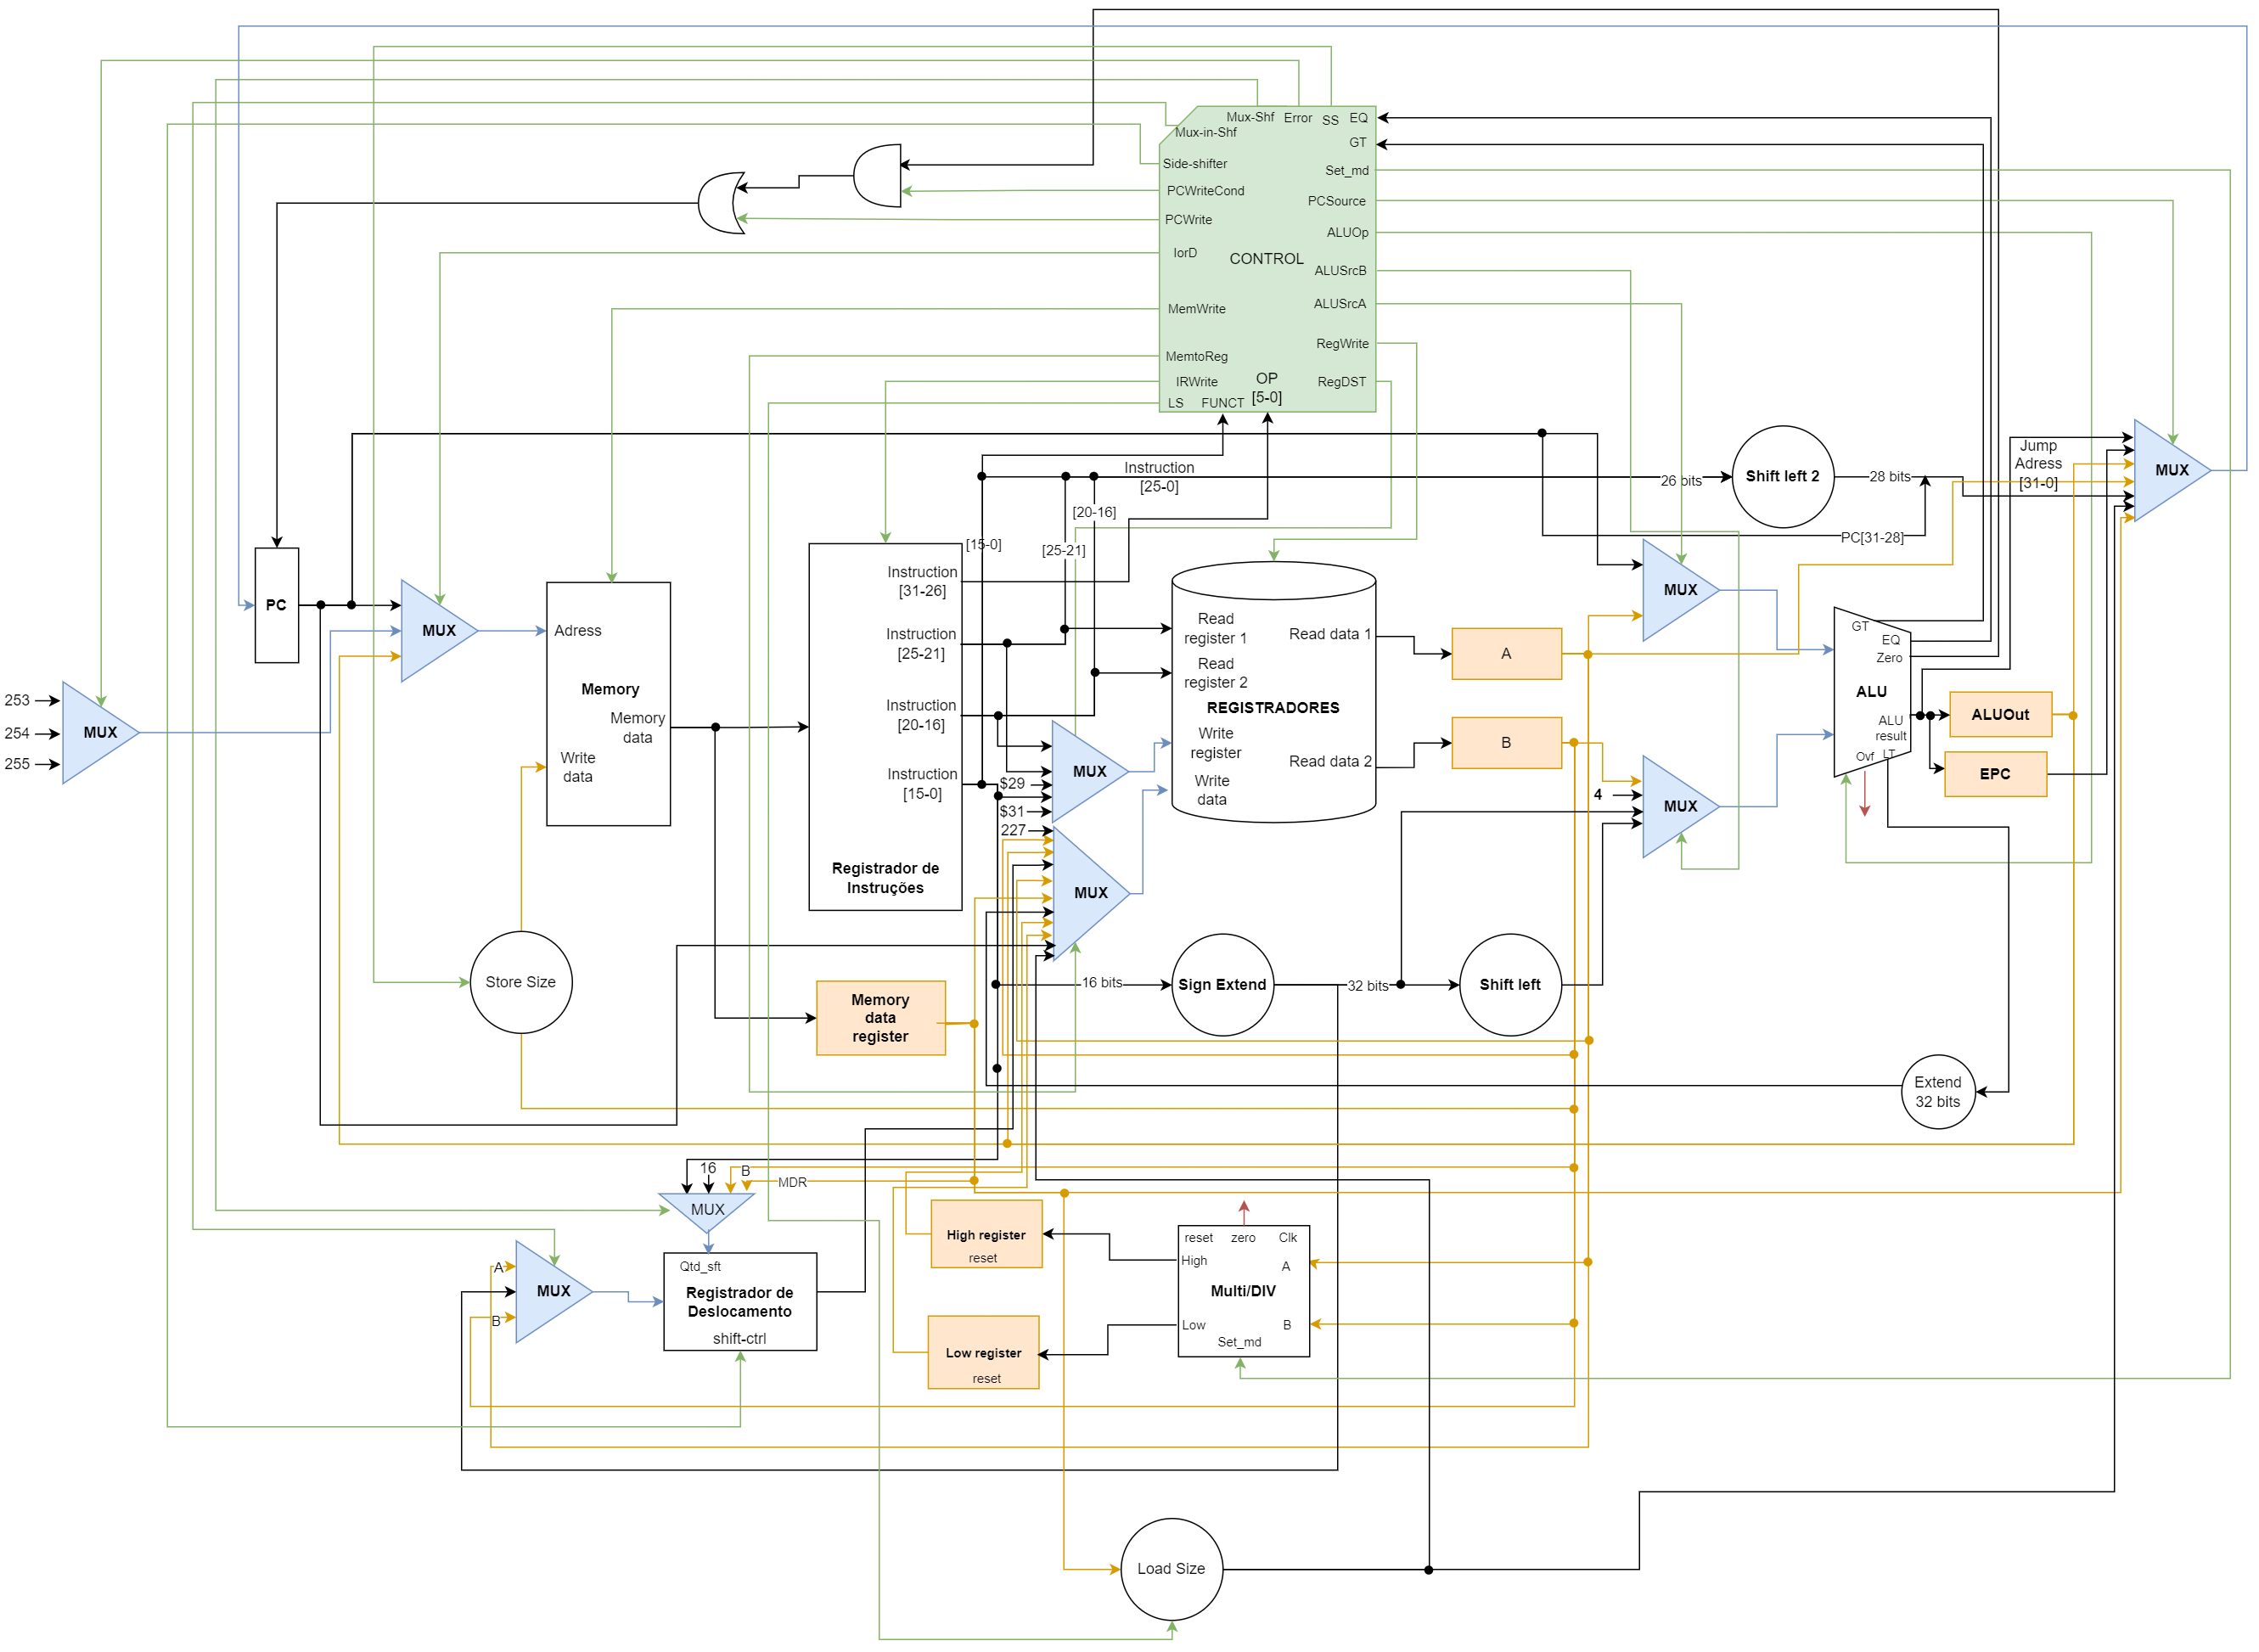
\includegraphics[width=1\textwidth]{figure/diagrama_bloco.png}
\caption{Diagrama de blocos} 
\label{fig:diagrama_blocos}
\end{figure}

A figura apresentada reflete a estrutura da unidade de processamento, onde as unidades estão representadas por blocos e as conexões por fios.

\newpage

\section{Examplo de subseções}

\subsection{subseção}

\textbf{Negrito - Exemplo de lista}

\begin{enumerate}
    \item Exemplo de 
    \item Lista.
\end{enumerate}

\newpage

\section{Exemplo de código}

Incrível "Hello World" em python em O(n!)

\lstinputlisting[caption={Exemplo de código em Python.}, label={lst:python_code}]{codes/hello_world.py}
